% To Do
% Allgemeinerer Start           |
% Quellen nach jedem Absatz     |
% Rechtschreibung :(            |
%

Heutzutage kommen sich die virtuelle und die realle Realität immer näher.
Angefangen von Virtual Reality, wo sich der Benutzer mithilfe einer VR-Brille in eine fiktive Welt begeben kann.
Bis hin zur Augmented Reality, in welcher virtuelle Gegenstände und Strukturen in der reallen Welt angezeigt werden können.
Es gibt neben BeamVR auch noch viele andere verschiedene Möglichkeiten um diese Konzepte umsetzen zu können.


%Das Konzept der Synchronisation von einem Gegenstand über den zwei besprochenen Realitäten ist nicht neu.
%Einer der bekanntesten Implementierungen des Konzepts ist Richie's Plank Experience.

\section{Richie's Plank Experience}
Ein Projekt welches zu einem Teil das gleiche Thema wie BeamVR behandelt, heißt Richie's Plank Experience, welches von TOAST VR PTY. LTD. entwickelt wurde.
Es handelt sich um ein Virtual Reality Spiel, dass auf der PlayStation 4, Oculus Quest und Microsoft Windows verfügbar ist.
Bei der Playstation wird auf das Sony exclusive PlayStation VR zurückgegriffen, während auf Windows entweder eine HTC Vive VR Brille oder die Valve Index verwendet werden kann.
(Quelle:~\cite{ToastGames_2021})

\subsection{Spielmodi}
Richie's Plank Experience, bietet dabei mehrere verschiedene Features in Form von Spielmodi an.
Diese Modi werden dem Spieler (ähnlich wie bei einer Stockwerkauswahl) in einem Aufzug dargestellt.
Wenn der Spieler einen Modus ausgewählt hat, fährt dieser auf das Hochhausdach.
Dort befindet sich dann der entsprechende Aufbau für den Modus.
Zur Verfügung stehen hierbei die Modi Plank, Sky Brush, Ground, Hero Academy und der Easter Egg Modus Nightmare.
(Quelle:~\cite{ToastGames_2021_Steam})

Im ersten Modus, welcher Plank genannt wird, befindet sich der Spieler weit oben auf einem Hochhaus.
Nach der Auswahl wird angeboten, dass sich am Ende des Balkens eine Belohnung befindet.
Man kann zwischen einem leeren Balken, Kuchen, Donuts und Kuchen mit darin versteckten Spinnen auswählen.
Nun befindet sich vor dem Aufzug nur mehr der Balken mit der vorher getroffenen Belohnung und rundherum der Abgrund.
Die Donuts und die beiden Kuchen können entweder gegessen oder heruntergeworfen werden.
(Quelle: ~\cite{ToastGames_2021_Steam})

In Sky Brush kann der Spieler, mithilfe eines kleinen Jetpacks, frei durch die Stadt fliegen.
Dabei wird eine Rauch-Spur hinterlassen welche, wie der Name des Modus schon andeutet, wie ein Pinsel in den Himmel malt.
Nun kann der Spieler, nach eigenem Belieben, verschiedene Kunstwerke erschaffen und betrachten.
(Quelle: ~\cite{ToastGames_2021_Steam})

Bei Hero Academy kann wieder zwischen mehreren Optionen auswählen.
Bei Fire Deck spielt man einen Superhelden welcher durch die Stadt fliegt und Feuer auf Häusern löschen muss.
Bei Air-Race fliegt man mit den Jetpacks durch Ringe welche als Checkpoints für ein Rennen dienen.
Wurden alle Ringe in richtiger Reihenfolge durchflogen, hat man das Rennen geschafft.
(Quelle: ~\cite{ToastGames_2021_Steam})

Im geheimen Modus Nightmare, welcher mithilfe von dem Code 666 erreicht werden kann, erlebt der Spieler eine kleine Abfolge von gruseligen Ereignissen.
(Quelle: ~\cite{ToastGames_2021_VivePort})

\subsection{Setup}

Damit man diese Modi, vor allem den Plank Modus, mit einem realen Balken spielen kann, muss mithilfe des Setups der Balken kalibriert werden.
Hierfür wird der Balken etwa in der Mitte der VR-Spielfläche platziert werden.
Nun sollten beide VR-Controller auf jeweils einem Ende des Balkens platziert werden, wie man auf der Grafik sehen kann.
~\ref{fig:beam_length_meassurement} %Balken Länge Einstellen

\begin {figure}
    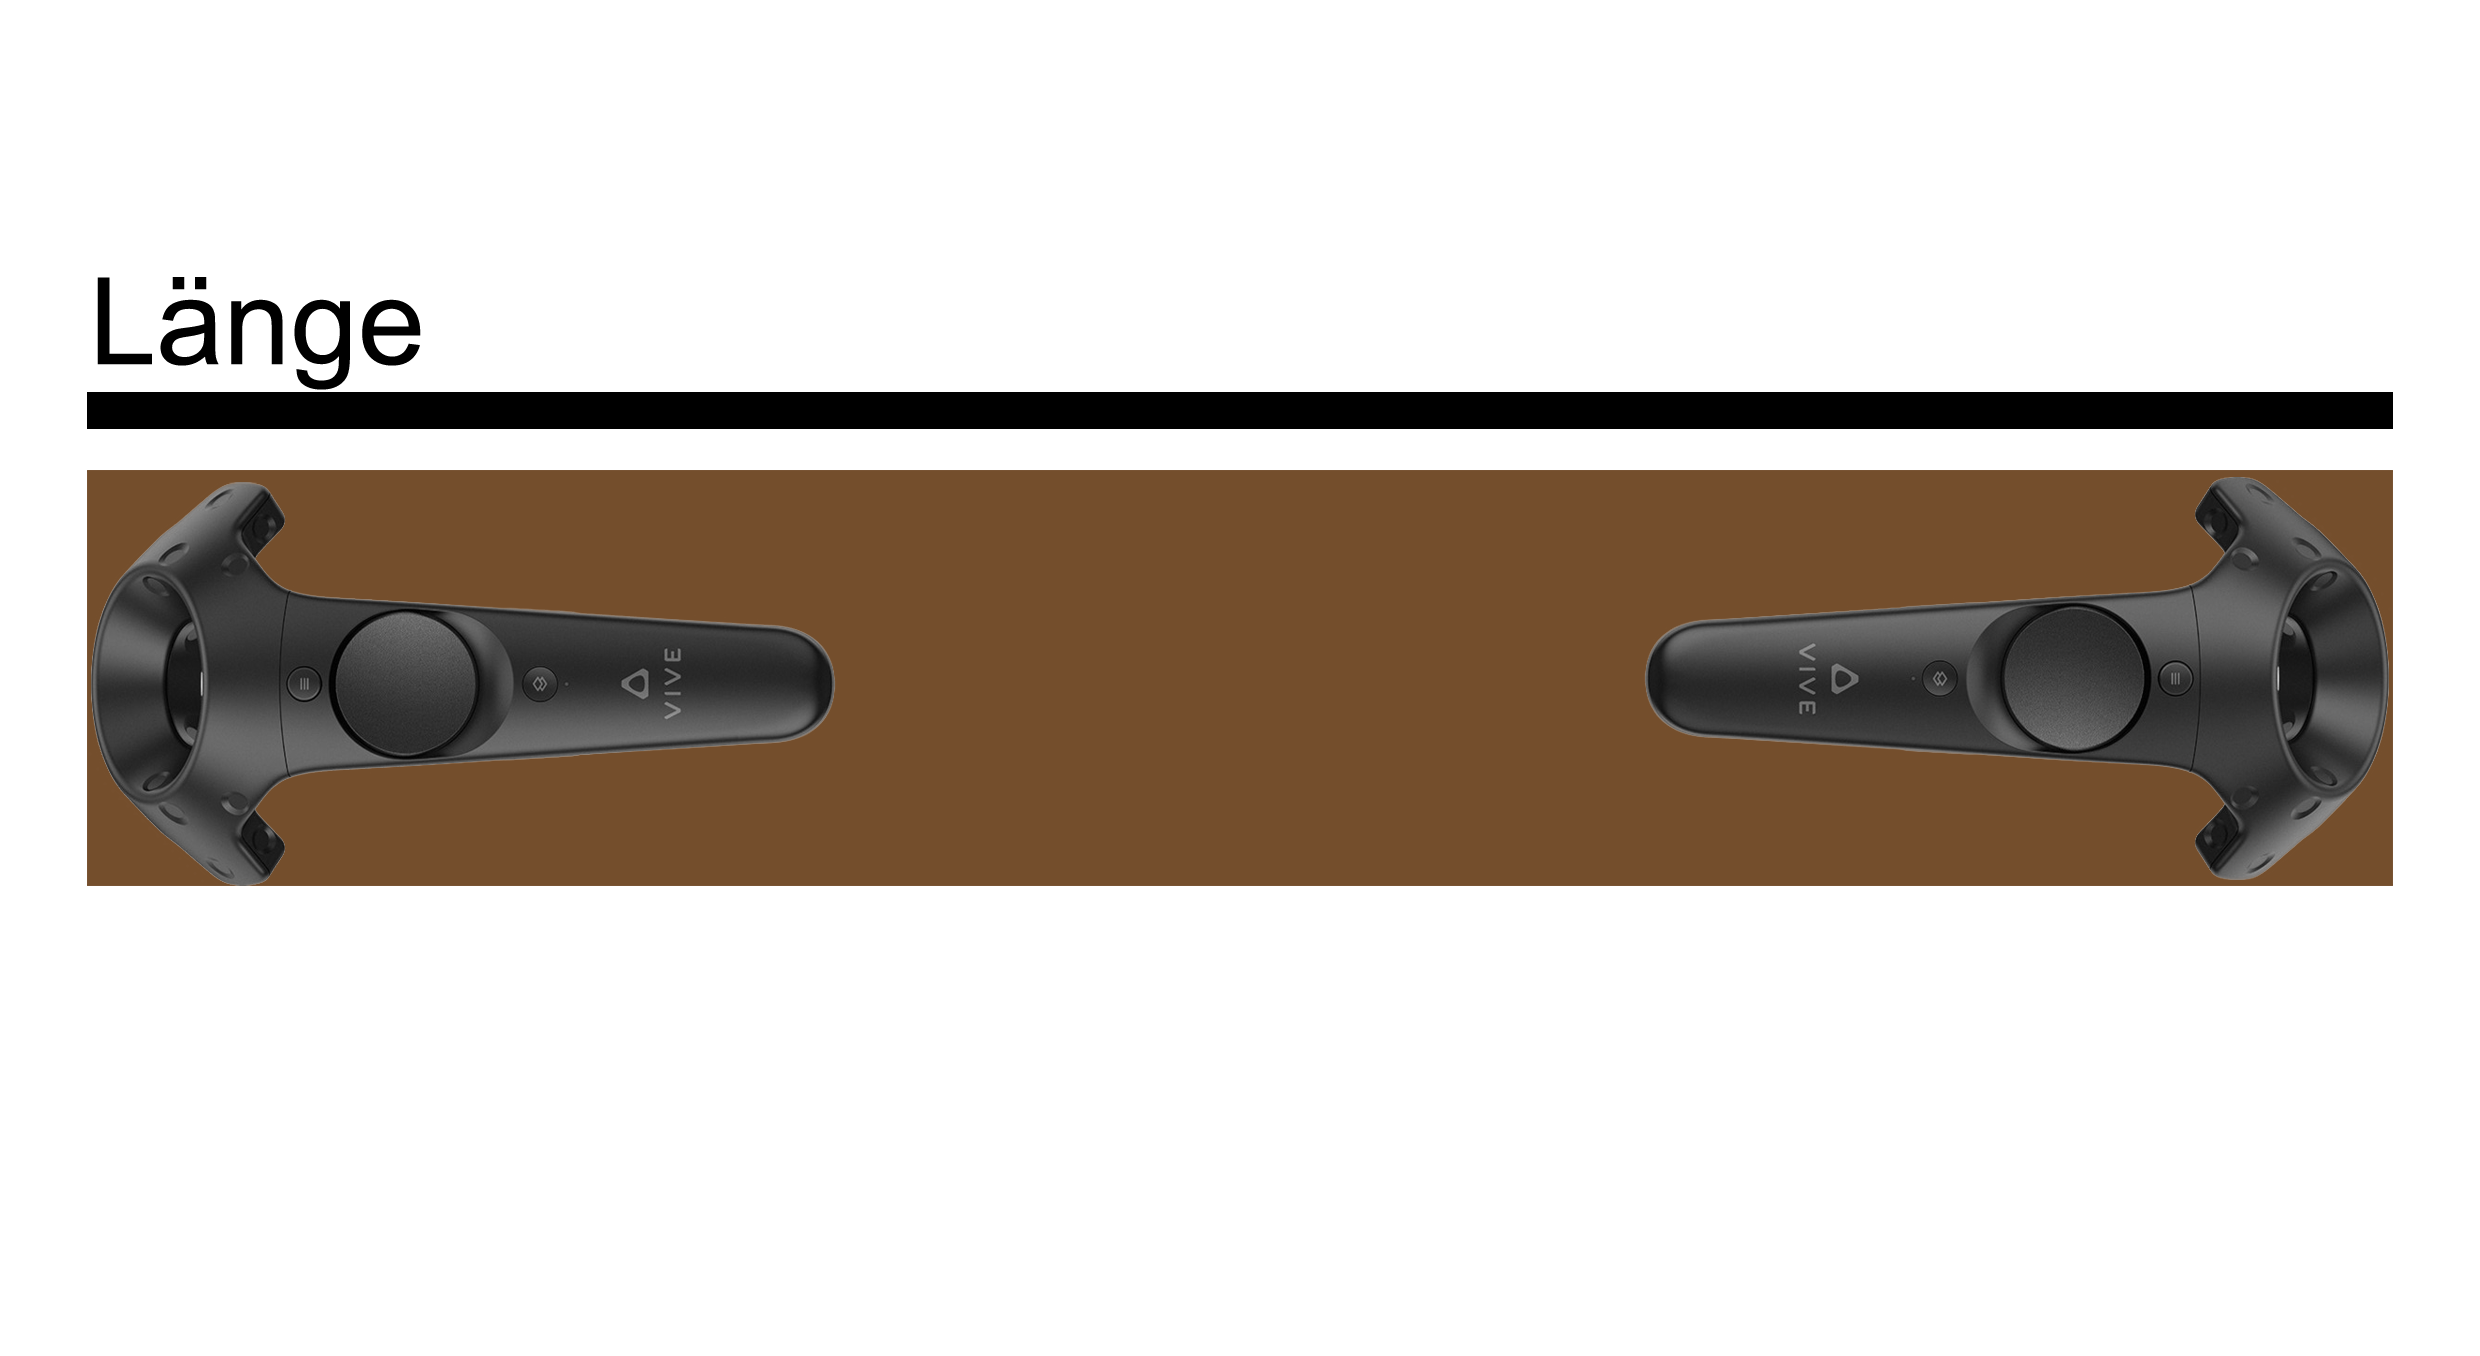
\includegraphics[scale=0.5]{pics/balken_laenge_messen}
    \caption{Laenge des Balken messen}
    \label{fig:beam_length_meassurement}
\end {figure}

Dadurch weiß die Applikation wie lange der Balken ist.
Man wird aufgefordert den Trigger des Controllers zu drücken, welche sich am Anfang des Balkens befindet, damit der Anfang und das Ende des Balkens bekannt gemacht wird.
%Grafik mit Setup Schritt 1



In Schritt zwei werden die Controller links und rechts vom Balken platziert und zeigen aufeinander.
Mit dieser Methode wird die Breite des Balkens gemessen.
%Grafik mit Setup Schritt 2
%\ref{id} %Balken Breite Einstellen

%\begin {figure}
%    \includeGraphics[scale=0.5]{pics/<image>}
%    \caption{des was unter dem bild stehen soll ohne abbildungsnummer}
%    \label{id}
%\end {figure}


Nun ist das Setup abgeschlossen und der Balken wird richtig in der virtuellen Welt angezeigt.
(Quelle:~\cite{ToastGames_2021_Setup}:])

\subsection{Spielwelt}
Alle Spielmodi befinden sich in einer Stadt, welche aus einer Vielzahl an verschiedenen Gebäuden besteht.
Die Architektur ist sehr vielfältig und realistisch gehalten.
Zwischen den Bauwerken befinden sich Straßen welche mit verschiedenen Pflanzen, z.B. Bäumen geschmückt sind.
Auf Fahrbahnen befinden Fahrzeuge, welche mit Schritttempo durch die Stadt fahren.

% // Vorerst raus gelöscht, weil ich die Verbesserung nicht lesen kann und es nicht bewiesen werden kann
%\subsection{Gravitation}
%NUR EINE THEORIE, HABE NICHTS IM INTERNET DAZU GEFUNDEN. Löschen? Wäre eigentlich wichtig.

%Die Immersion in dem Spiel wird nochmals verstärkt, indem man auch von dem Balken stürzen kann.
%Dies wurde gelöst indem einfach die Distanz auf der X- und Z- Koordinate zum Balken gemessen wurde, hierbei wird der Höhenunterschied nicht betrachtet.
%Wenn der Spieler sich nun zu weit von dem Balken entfernt, bewegt sich dieser entlang der Y-Achse Richtung Boden, er fällt also vom Balken.


% QUELLEN Wo schreibe ich die nochmal hin?
%https://toast.games/
%https://www.youtube.com/watch?v=L088mfO2Ieg
%https://www.bevirtual.be/games/vr-experience/richies-plank-experience/
%
%
%
%


%\lipsum[4] Citing \cite{InfH} properly.
%
%Was ist eine \gls{guid}?
%Eine \gls{guid} kollidiert nicht gerne.%
%
%Kabellose Technologien sind in abgelegenen Gebieten wichtig \cite{APCW2006}.
